\newpage
\chapter{Dynamische Algorithmen zur Ausrei�er Erkennung}
\label{chap:dynamic}

In diesem Kapitel werden zwei Algorithmen zur dynamischen Erkennung von Ausrei�ern vorgestellt. Hierbei handelt es sich um den NetSimile (vgl. \autoref{sec:ns}) und den MIDAS (vgl. \autoref{sec:midas}) Algorithmus. Dynamische Algorithmen k�nnen im Gegensatz zu statischen Algorithmen, Ausrei�er in Echtzeitdaten finden. Dies kann in der Praxis sehr wichtig sein, da Ausrei�er m�glichst schnell gefunden werden m�ssen um die daraus resultierenden finanzielle Sch�den abzuwenden.  Im Zuge des Forschungsprojekts werden die dynamischen Algorithmen ebenfalls auf den unterschiedlichen Input, je nach Anwendungsfall, angepasst. Dadurch wird gew�hrleistet, dass diese Algorithmen ebenso wie die statischen Algorithmen aus \autoref{chap:static} mit unterschiedlichen Datentypen umgehen k�nnen. In den Tests des Forschungsprojekts werden die Algorithmen auf Netzwerk- und Zeitreihendaten angewandt.

\section{Umwandlung der Daten in ein Netzwerk}
\workTodo{Ich dachte in einen Graphen?????}
Bevor die dynamischen Algorithmen auf die Zeitreihendaten angewendet werden k�nnen, m�ssen diese in Graphen transformiert werden. Dabei funktioniert die Umwandlung der Daten �hnlich wie bei statischen Algorithmen (vgl. \autoref{sec:trsnsNeti}). Der einzige Unterschied hierbei ist, dass jeweils schrittweise kleine Abschnitte der Daten in Netzwerke umgewandelt werden. Nachfolgend wird dies an einem Beispiel n�her veranschaulicht. Ein Temperatursensor liefert jede Sekunde einen Wert. Sobald 100 Werte des Sensors eingegangen sind, erfolgt die Umwandlung dieser Daten in ein Netzwerk unter Verwendung von \autoref{eq:euklidianDist}. Dieser Vorgang wiederholt sich anschlie�end immer wieder. Der Wert f�r die L�nge der Abschnitte ist hierbei frei w�hlbar und kann als Parameter �bergeben werden. Insofern die Zeitreihe eine Saisonalit�t besitzt, bietet es sich an diese f�r die L�nge der Abschnitte zu verwenden. In einem letzten Schritt werden anschlie�end die Netzwerkdaten in eine Datei geschrieben. Dieser Schritt ist aufgrund der Art und Wei�e, wie die Algorithmen implementiert sind notwendig. In \autoref{sec:trsnsNeti} ist graphisch dargestellt wie die Umwandlung der Daten in ein Netzwerk funktioniert. 

\begin{figure}[H]
	\centering
	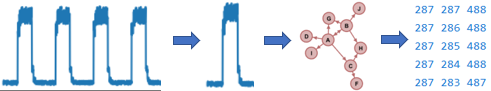
\includegraphics[width=13cm]{fig/tsToNet/tsToCsv}
	\caption{Umwandlung einer Zeitreihe in ein Netzwerk. Bei dem Netzwerk handelt es sich hierbei um ein Symbolbild.}
	\label{img:tsToNet}
\end{figure}

\label{ssec:trsnsCSV}
Die verschiedenen Algorithmen erfordern unterschiedliche �bergabeformate. Aus diesem Grund werden anschlie�end kurz die Besonderheiten erkl�rt, auf welche dabei geachtet werden muss. \\
\textbf{NetSimile: } Das �bergabeformat f�r den NetSimile Algorithmus ist in \autoref{img:tsToNet} ganz rechts dargestellt. Jede Zeile stellt hierbei eine Kante des Netzwerks dar. Bei der ersten Spalte handelt es sich um den Ursprungsknoten der Kante, bei der zweiten Spalte um den Zielknoten und bei der letzten Spalte um die Gewichtung.\\
\textbf{MIDAS: } Beim MIDAS Algorithmus ist es nicht m�glich die Gewichtung der Kanten direkt an den Algorithmus zu �bergeben. Es ist jedoch m�glich die Gewichtung der Kanten indirekt an den Algorithmus zu �bergeben. Dazu wird die gleiche Kante mehrmals in Abh�ngigkeit der Gewichtung an den Algorithmus �bergeben. In \autoref{img:tsToNetMiData} ist ein  kleiner Ausschnitt einer Datei f�r den MIDAS dargestellt.

\begin{figure}[H]
	\centering
	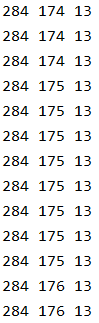
\includegraphics[width=2cm]{fig/tsToNet/midasData}
	\caption{Datensatz Midas. 1Spalte: Ursprungsknoten, 2Spalte: Zielknoten, 3Spalte: Abschnitt}
	\label{img:tsToNetMiData}
\end{figure}
\textbf{MIDAS-R: }. Die Berechnungen f�r den MIDAS-R Algorithmus sind im Verh�ltnis zum MIDAS Algorithmus umfangreicher. Insofern f�r den MIDAS-R Algorithmus die gleichen Daten verwendet werden wie f�r den MIDAS Algorithmus, ben�tigen die Berechnungen sehr lange. Aus diesem Grund wurde eine Hauptkomponenten Zerlegung durchgef�hrt, um die Gr��e der Adjazenzmatrix zu verringert. Es entsteht ein kleineres Netzwerk, welches an den MIDAS-R Algorithmus �bergeben werden kann. 
\label{ssec:trsnsMidasR}


\newpage
\section{Netsimile}
\label{sec:ns}

\subsection{Grundlagen}
\label{ssec:ns-gl}

Netsimile ist ein skalierbarer Algorithmus zur Erkennung von �hnlichkeiten, sowie Anomalien in Netzwerken unterschiedlicher Gr��en. Hierf�r wird der Datensatz in gleich gro�e Zeitintervalle unterteilt, um die daraus resultierenden Graphen auf unterschiedliche Merkmale zu untersuchen. Die Merkmale sind hierbei strukturelle Eigenschaften der einzelnen Knoten wie bspw. die Dichte eines Knotens oder die Anzahl an Nachbarn in einem Ego-Netzwerk. Die Signatur ergibt sich aus den einzelnen Aggregationen der Knoten wie bspw. der Median aus der Dichte der jeweiligen Knoten. So entsteht bspw. aus sieben Merkmalen und f�nf Aggregationen ein Signaturvektor mit 35 verschiedenen Signaturen. So erm�glicht der Signarturvektor die Beschreibung als auch den Vergleich der einzelnen Graphen. F�r den Vergleich wird die Canberra Distanz aus den beiden Signaturvektoren zweier zeitlich nebeneinander liegenden Graphen berechnet. \citep[vgl.][S.~1]{Netsimile}

Als Input f�r diesen Algorithmus wird eine Menge von $k$-anonymisierten Netzwerken mit beliebig unterschiedlichen Gr��en, die keine �berlappenden Knoten oder Kanten besitzen sollten, herangezogen werden. Das Resultat sind Werte f�r die strukturelle �hnlichkeit oder Abstands eines jeden Paares der gegebenen Netzwerke bzw. ein Merkmalsvektor f�r jedes Netzwerk. \citep[vgl.][S.~1]{Netsimile}

Netsimile durchl�uft drei Schritte, die im Folgenden erl�utert werden.

\subsubsection{Extrahierung von Merkmalen}
F�r jeden Knoten $i$ werden, basierend auf ihren Ego-Netzwerken, die folgenden Merkmale generiert:


\begin{description}
	\item[$\overline{d}_i = |N(i)|$]\hfill\\ Die Anzahl der Nachbarn (d.h. Grad) von Knoten $i$, wobei $N(i)$ die Nachbarn von Knoten $i$ beschreibt.
	\item[$\overline{c}_i$]\hfill\\ Der Clustering-Koeffizient von Knoten $i$, der als die Anzahl von Dreiecken, die mit Knoten $i$ verbunden sind, �ber die Anzahl von verbundenen Dreiecken, die auf Knoten $i$ zentriert sind, definiert ist.
	\item[$d_{N(i)}$]\hfill\\ Die durchschnittliche Anzahl der Nachbarn von Knoten $i$, die zwei Schritte entfernt sind. Dieser wird berechnet als \workTodo{Paper Seite 2 unten Formel einf�gen}
	\item[$c_{N(i)}$]\hfill\\ Der durchschnittliche Clustering-Koeffizient von $N(i)$, der als \workTodo{Paper Seite 2 unten Formel einf�gen} berechnet wird.
	\item[$|E_{ego(i)}|$]\hfill\\ Die Anzahl der Kanten im Ego-Netzwerk vom Knoten $i$, wobei $ego(i)$ das Ego-Netzwerk von $i$ zur�ckgibt.
	\item[$|E^{\circ}_{ego(i)}|$]\hfill\\ Die Anzahl der von $ego(i)$ ausgehenden Kanten. 
	\item[$|N(ego(i))|$]\hfill\\ Die Anzahl von Nachbarn von $ego(i)$. 
\end{description}

\subsubsection{Aggregierung von Merkmalen}
Im n�chsten Schritt wird f�r jeden Graphen \textit{$G_j$} eine $Knoten \times Merkmal$-Matrix $F_{G_j}$ zusammengefasst. Dieser besteht aus den Merkmalsvektoren aus Schritt 1.
Da der Vergleich von $k$-ten $F_{G_j}$ sehr aufw�ndig ist, wird f�r jede $F_{G_j}$ ein Signaturvektor $\vec{s}_{G_j}$ ausgegeben. Dieser aggregiert den Median, den Mittelwert, die Standardabweichung, die Schiefe, sowie die Kurtosis der Merkmale aus der Matrix.  

\subsubsection{Vergleich der Signaturvektoren}
\label{sec:ns-gl-cd}

F�r die Ausrei�ererkennung werden die letzten drei Graphen anhand der Canberra-Distanz-Funktion, die als �hnlichkeitsma� dient, herangezogen. Steigt die Canberra Distanz zwischen zwei Graphen oberhalb des Thresholds so wird dies im Algorithmus festgehalten. Falls der darauf folgende Graph ebenfalls oberhalb des Thresholds liegt, so wird dieser als Ausrei�er definiert. Dadurch wird die Anzahl der Ausrei�er reduziert, damit nur diejenigen identifiziert werden, bei denen ein Trend hin zu einem abnormalen Verhalten erkennbar ist.

Der Algorithmus arbeitet dabei dynamisch, da die Signaturen der Graphen in einzelne Teil-Berechnungen aufgesplittet und zwischengespeichert werden k�nnen, ohne das eine Neuberechnung notwendig ist. Der Threshold wird aus dem Median und dem Mean berechnet, welche ebenfalls Zwischengespeichert werden k�nnen und nach Bedarf um weitere Graphen erg�nzt werden k�nnen.

\FloatBarrier

\subsection{Anwendung des Algorithmus auf Netzwerkdaten}
\label{sec:ns-ext}
Beim ersten Versuch den Algorithmus auf Netzwerkdaten anzuwenden, wurde folgende Probleme festgestellt:

Der Algorithmus verwendet eine Bibliothek \textit{igraph}, welche Kanten zwischen zwei Knoten nur einmalig hinzuf�gen kann. Beim Eliminieren der Duplikate w�rde aber ein Drittel des Datensatzes nicht ber�cksichtigt werden, wodurch wertvolle Informationen bei der Ausrei�ererkennung verloren gehen w�rden. Aus diesem Grund wurden die Netzwerkdaten soweit angepasst, dass Mehrfachverbindungen zwischen zwei Kanten aufsummiert werden und als Gewichtung dieser Kante hinzugef�gt wird. 

\begin{lstlisting}[language=Python, caption=Gewichtung als neues Feature, label=lst:netsimile:code1]
for i in range(len(e_list)): 
	g.add_edge(e_list[i][0], e_list[i][1], weight=e_list[i][2])
\end{lstlisting}

Dadurch kann der Datensatz zum einen vollst�ndig analysiert werde und zum anderen konnte dadurch ein weiteres Feature hinzugef�gt werden, dass durch die f�nf verschiedenen Aggregationen den Signaturvektor um diese f�nf Werte erweitert.

Dadurch das der Datensatz zuerst eingelesen und in einen Graphen transformiert wird und anschlie�end aus dem Graphen die jeweiligen Features extrahiert werden, verliert der Algorithmus extrem an Performanz. Des weiteren wird im ersten Schritt der maximale Knoten-Wert als Gr��e des Graphens �bergeben. Wird bspw. f�r jeden Mitarbeiter eine eigene ID �bergeben und die inkrementell erh�ht, so kann es sein, dass aus einem Netzwerk mit 20 verschiedenen Knoten ein Graph erzeugt wird, der 1000 Knoten erzeugt, weil eine ID mit dem Wert 1000 vorhanden ist. Dadurch b��t die Performanz an Geschwindigkeit ein, da Iterationen nicht �ber die 20 Knoten durchgef�hrt werden, sondern �ber 1000. Hier muss entweder der Datensatz vorab angepasst werden, indem die IDs neu vergeben werden oder der Algorithmus muss grundlegend neu aufgebaut werden.

Da der Fokus auf der Anwendung von Zeitreihen liegt, wird die Optimierung erst in diesem Abschnitt erl�utert.



Das Problem hierbei ist, dass jeder Knoten eines Graphens die gleichen Features beinhalten w�rde. Dadurch w�rden die Aggregationen �berfl�ssig werden und der Signaturvektor auf sieben Features schrumpfen. Die Bildung von Cluster-Features w�re demnach nur noch bedingt m�glich und die Betrachtung an Nachbarn, unabh�ngig ob im Ego-Netzwerk oder im gesamten Netzwerk w�rde sich die Gesamtanzahl an Knoten ann�hern. Im Folgenden wird das Verh�ltnis der Features zum Durchschnitt dargestellt.

\subsubsection{Anwendung auf ENRON-Datensatz}
\label{sec:ns-enron}

Da der Enron Datensatz ebenfalls von einem anderen Paper analysiert und ver�ffentlicht wurde, k�nnen die dort erkannten Ausrei�er zum Vergleich in Form eines gelabelten Datensatz verwendet werden.
Betrachtet man in diesem Kontext den Aurei�erscore, ist gut zu erkennen, dass der Ausrei�er Ende 2001 als alleiniger herausstechender Ausrei�er auch im Ergebnis wiederzufinden ist. Grundlegend ist aber auch zu erkennen, dass die Ausrei�er sich nur sehr wenig voneinander unterscheiden, wodurch eine Klassifizierung innerhalb des Ausrei�erscores sich als schwierig erweist. Die Extrahierung weiterer Features k�nnte hier eventuell aushelfen, wobei dies nicht im Rahmen dieses Forschungsprojektes behandelt werden soll, da der Fokus auf Zeitreihen liegt. Zwecks Performanz konnte der Datensatz innerhalb von zwei Minuten analysiert werden.

\begin{figure}[H]
	\centering
	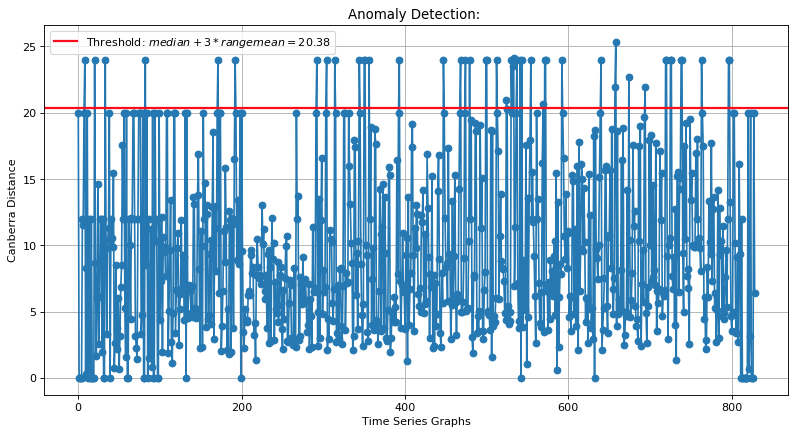
\includegraphics[height=0.6\linewidth,width=\linewidth]{fig/netsimile/anomalie_3}
	\caption{Ausrei�er Score Enron Datensatz}
	\label{img:netsimile:anomalie_3}
\end{figure}

\begin{figure}[H]
	\centering
	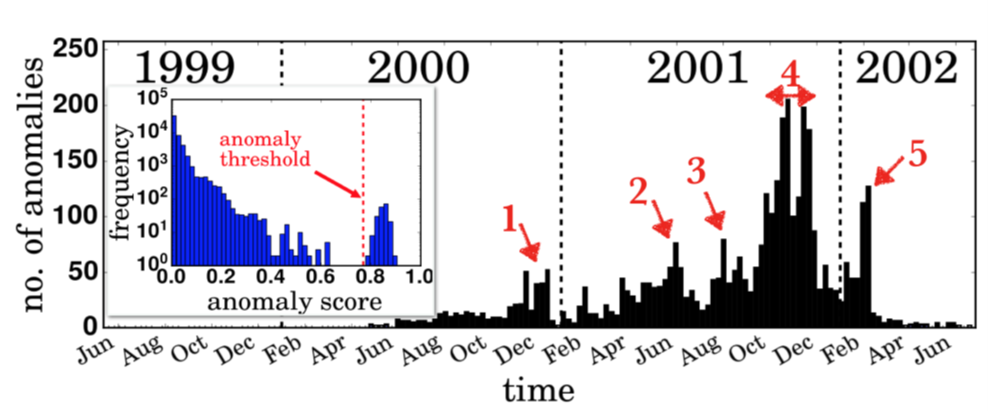
\includegraphics[height=0.6\linewidth,width=\linewidth]{fig/sedanspot}
	\caption{\workTodo{Sedanspot Caption}}
	\label{img:sedanspot}
\end{figure}

Betrachtet man die Differenz aus dem Durchschnitt der Signaturvektoren und den der Ausrei�ergraphen in einer Headmap kann man erkennen, dass die Ausrei�er vorwiegend durch besonders gro�e Ego-Netzwerke und einer hohen Anzahl an E-Mails verschuldet ist.



\begin{figure}[H]
	\centering
	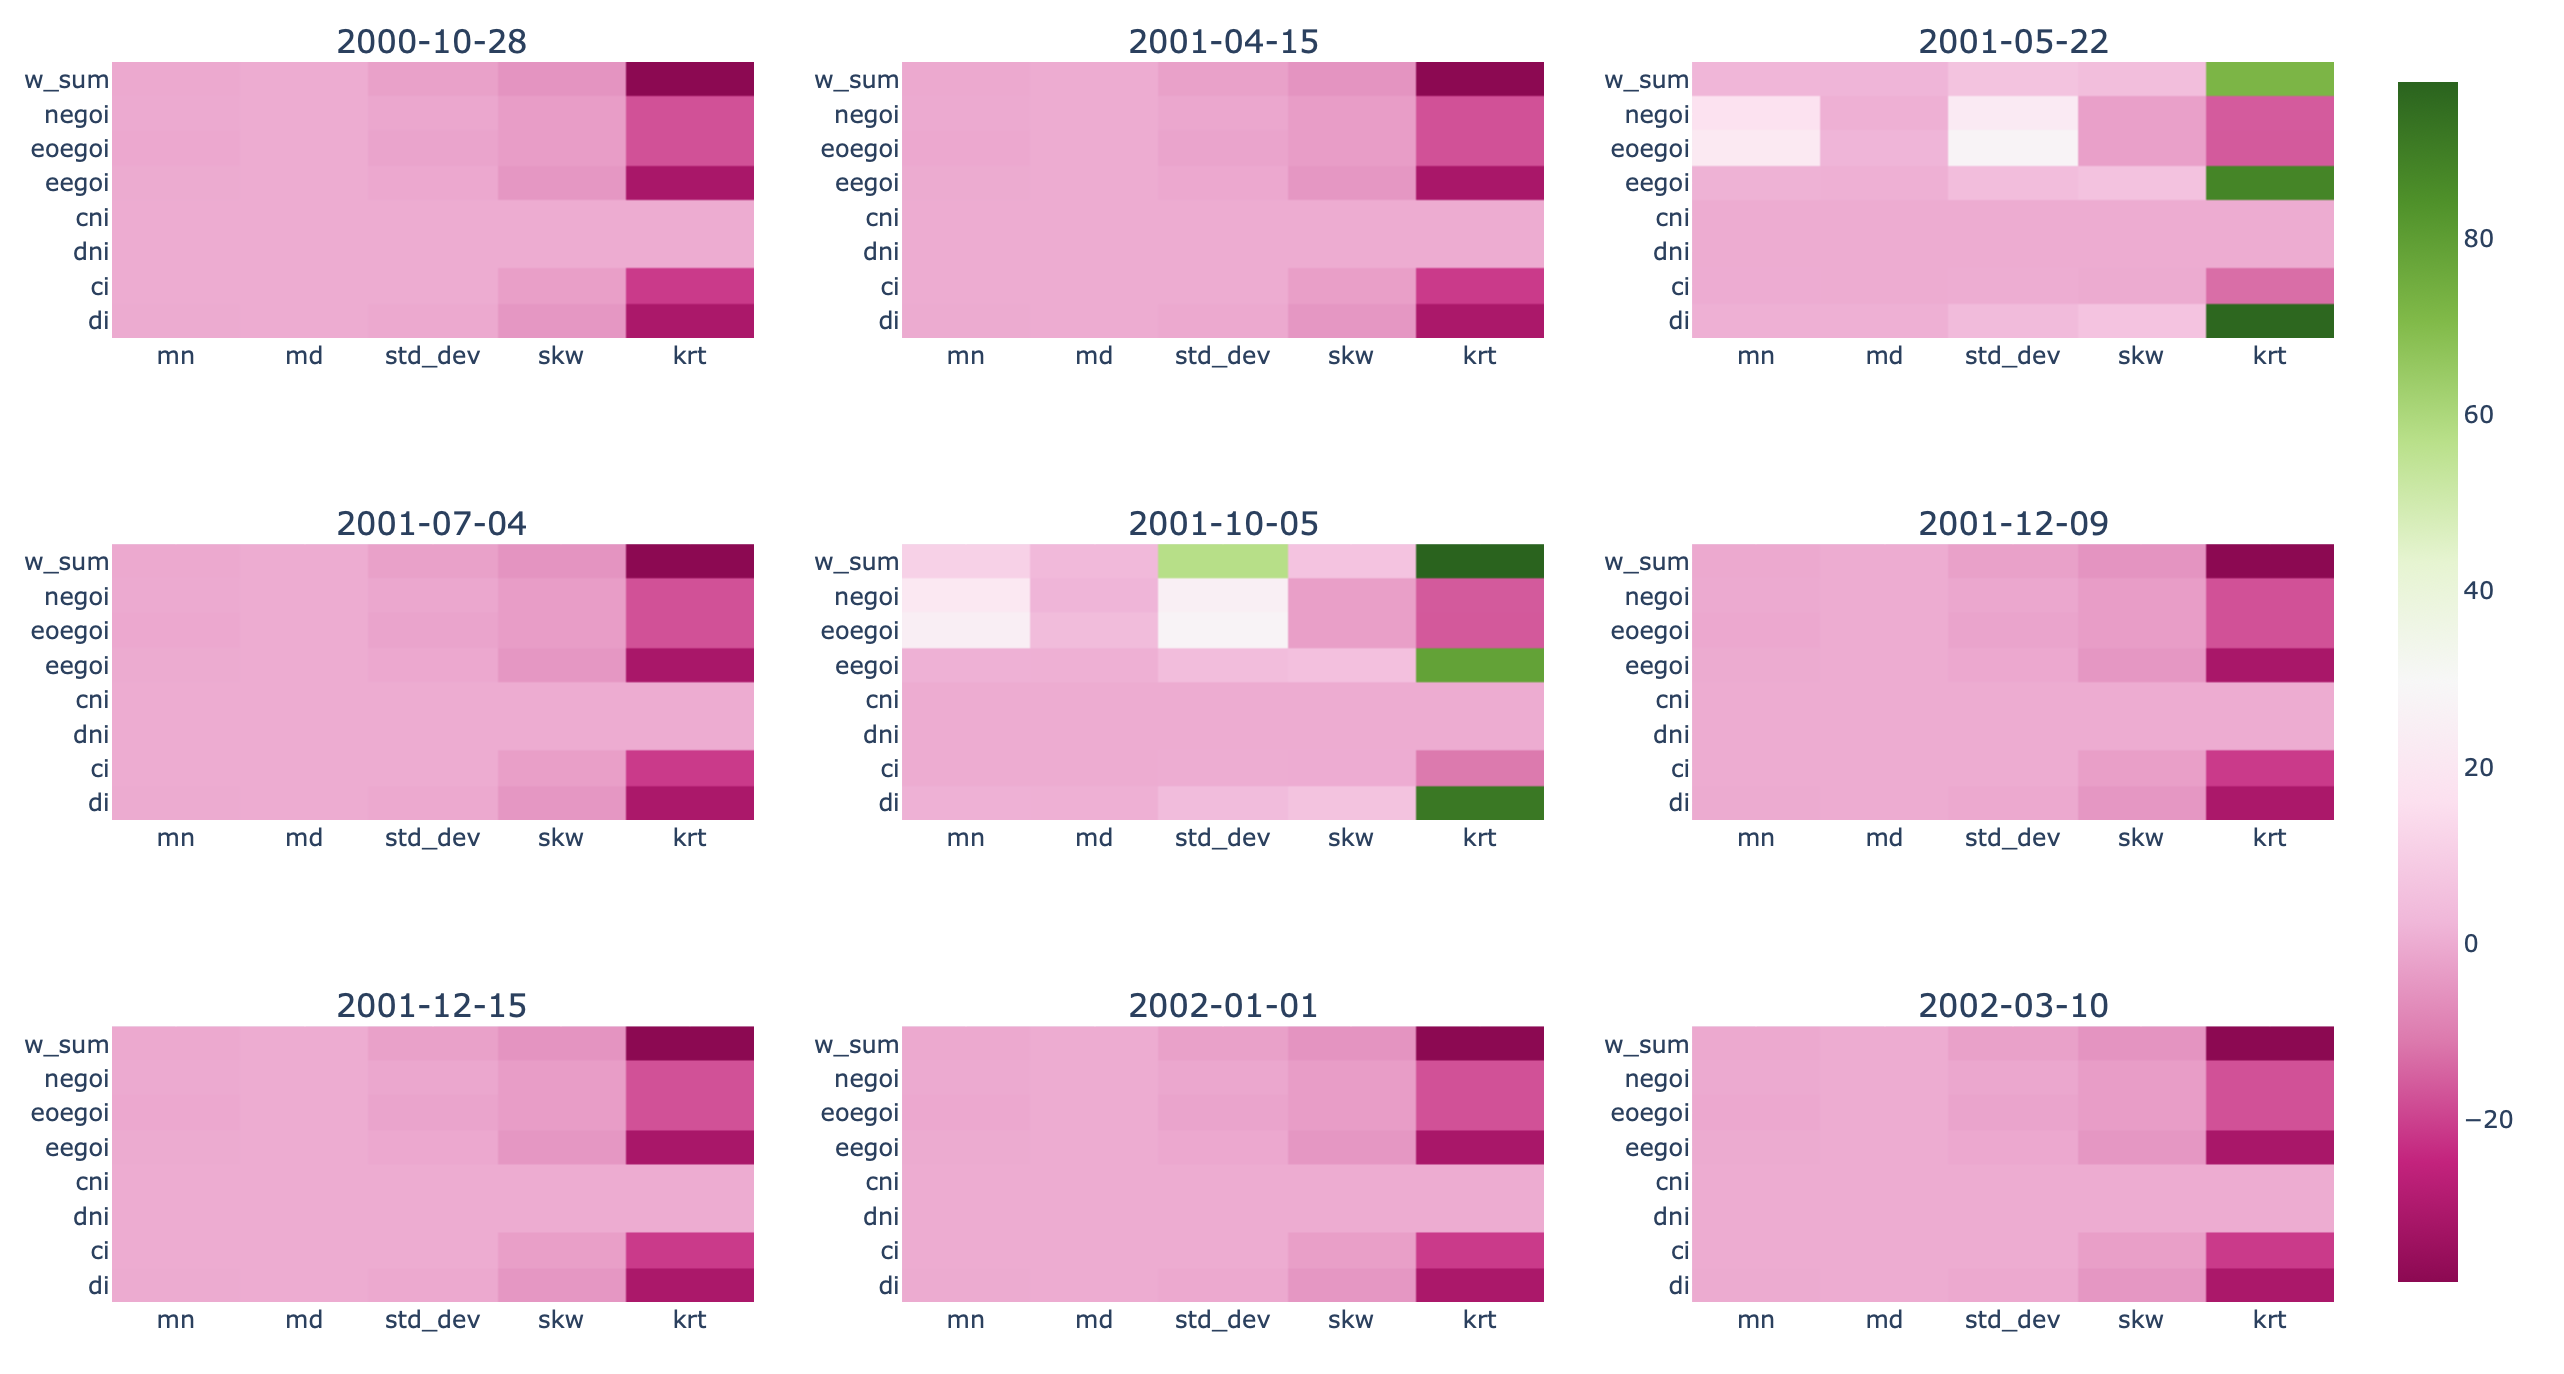
\includegraphics[height=0.8\linewidth,width=\linewidth]{fig/netsimile/heatmap_3}
	\caption{Darstellung der Ausrei�er in Heatmaps}
	\label{img:netsimile:heatmap_3}
\end{figure}

\subsubsection{Anwendung auf DARPA-Datensatz}
\label{sec:ns-darpa}

Beim Darpa Datensatz k�nnen die Aurei�er besser klassifiziert werden. Die Gr�nde k�nnen hierbei auf die Gr��e und Vielfalt des Datensatzes zur�ckgef�hrt werden. Der Enron Datensatz hat eine Gr��e von 1MB und rund 50.000 Kanten. Der Darpa Datensatz hingegen hat eine Gr��e von 50 MB mit 4.5 Mio Kanten. Die Berechnung hat dabei eine L�nge von 3h. Haben wir bei der Dateigr��e den Faktor 50 und bei der Kantenanzahl den Faktor 90, so ist bei der Berechnungszeit der Faktor 90 wiederzufinden. Betrachtet man die Laufzeit, so kann eine lineare Abh�ngigkeit zwischen Kantenanzahl und der ben�tigten Berechnungszeit festgestellt werden.

\begin{figure}[H]
	\centering
	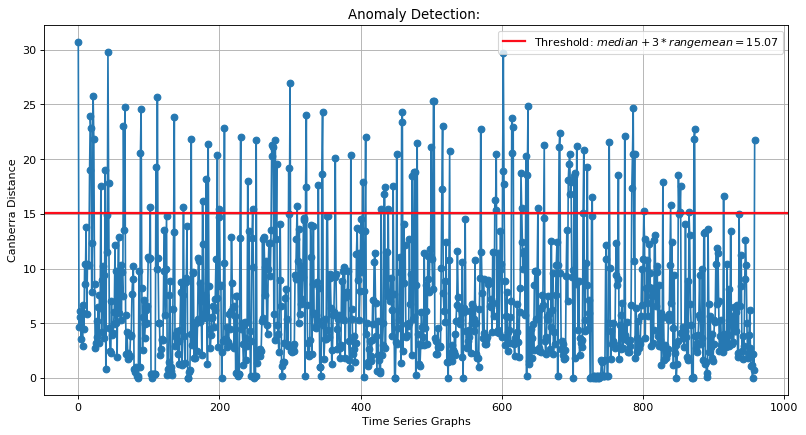
\includegraphics[height=0.6\linewidth,width=\linewidth]{fig/netsimile/anomalie_4}
	\caption{Ausrei�er Score DARPA}
	\label{img:netsimile:anomalie_4}
\end{figure}

\subsection{Anwendung des Algorithmus auf Zeitreihen}
\label{sec:ns-ts-1}

Wird der Algorithmus auf Zeitreihen anwendet, entsteht folgendes Problem. Bei der Transformation der Daten entstehen vollst�ndige Graphen, wodurch die strukturellen Eigenschaften identisch werden, sowie die daraus resultierenden Merkmale, wie in der Abbildung verdeutlicht werden soll. 

\usetikzlibrary{graphs,graphs.standard}
\begin{figure}[H]
	\centering
	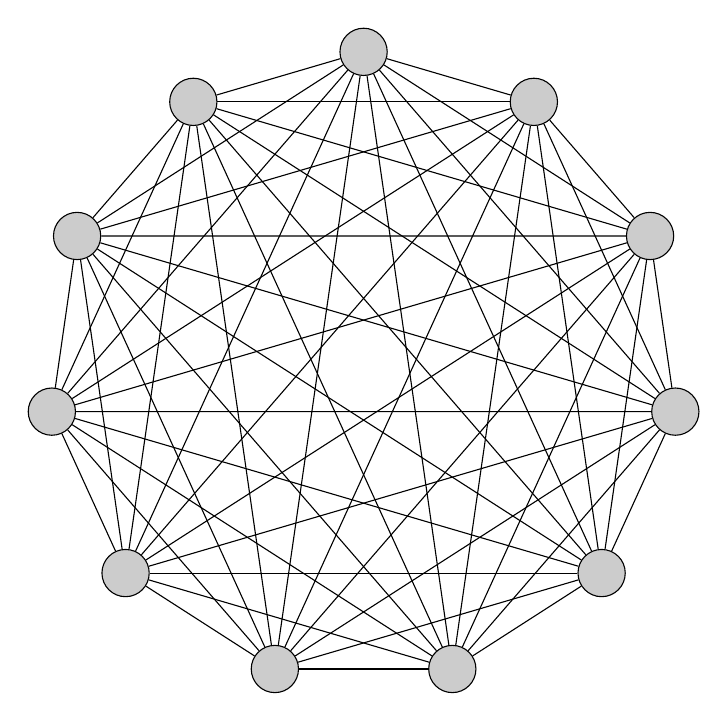
\begin{tikzpicture}
		\graph[nodes={draw, circle,fill=black!20,minimum size = 6mm}, clockwise, empty nodes, radius=4cm, n=11] { subgraph K_n };
	\end{tikzpicture}
	\caption{Vollst�ndiger Graph mit 11 Knoten}
	\label{img:netsimile:graph_11}
\end{figure}

So hat bspw. das Feature $|E^{\circ}_{ego(i)}|$ keine Aussagekraft in einem vollst�ndigen Graphen, da jeder Knoten die gleiche Anzahl Kanten in seinem Ego-Netzwerk aufweist. Subtrahiert man also vom durchschnittlichen Signaturvektor aller Graphen die einzelnen Signaturvektoren, so erh�lt man den Wert 0 f�r alle Headmaps sowie den Threshold (vgl. \autoref{img:netsimile:heatmap_1}, \autoref{img:netsimile:anomalie_1}).

Somit m�ssen hier f�r diese Art von Graphen andere Features extrahiert werden. Au�erdem ist die Laufzeit in gro�en Datens�tzen, wie bspw. dem Darpa-Datensatz mit 3h Berechnungszeit nicht gerade performant.

Aus diesem Grund werden aus dem Netsimile lediglich die Ans�tze der Feature Extrahierung �bernommen, die Aggregationen ,die Distanzbildung zweier Signaturvektoren, sowie der Threshold f�r die Ausrei�eridentifizierung.

Das hei�t die Netzwerke der Zeitreihe werden nicht in ein Graphen Objekt umgewandelt, sondern als Adjazenzmatrix gespeichert. Dadurch k�nnen die Features deutlich effizienter berechnet werden. Zudem werden lediglich Features verwendet, die f�r vollst�ndige Graphen geeignet sind. Dabei werden folgende Features neu eingef�hrt:



\workTodo{n-te Wurzel bei Formel f�r Geometrischen Mittelwert}
\begin{description}
	\item[$\sum_{i=1}^{n} x_i $]\hfill\\ Summe der Kantengewichte eines Knoten.
	\item[$\frac{1}{n}\sum_{i=1}^{n} x_i $]\hfill\\ Arithmetisches Mittel der Kantengewichte eines Knoten.
	\item[$ \sqrt{\prod\limits_{i = 1}^{n} x_i} $]\hfill\\ Geometrisches Mittel der Kantengewichte eines Knoten.
	\item[$
	x(p) =
	\begin{cases}
		\frac{1}{2}x_(np) +       & \quad \text{if } n \text{ is even}\\
		-(n+1)/2  & \quad \text{if } n \text{ is odd}
	\end{cases}
	$]\hfill\\ Geometrisches Mittel der Kanten mit den 10\% h�chsten Kantengewichten. 
	\item[$\frac{1}{n}\sum_{i=1}^{n} x_i$]\hfill\\ Geometrisches Mittel der Kanten mit den 20\% h�chsten Kantengewichten. 
\end{description}

Von diesen Features wurde dann auch den Median, den Mittelwert, die Standardabweichung, die Schiefe, sowie die Kurtosis berechnet. Dadurch konnten erste Ausrei�er in der Zeitreihe gefunden werden (vgl. \autoref{img:netsimile:anomalie_2}).

\begin{figure}[H]
	\centering
	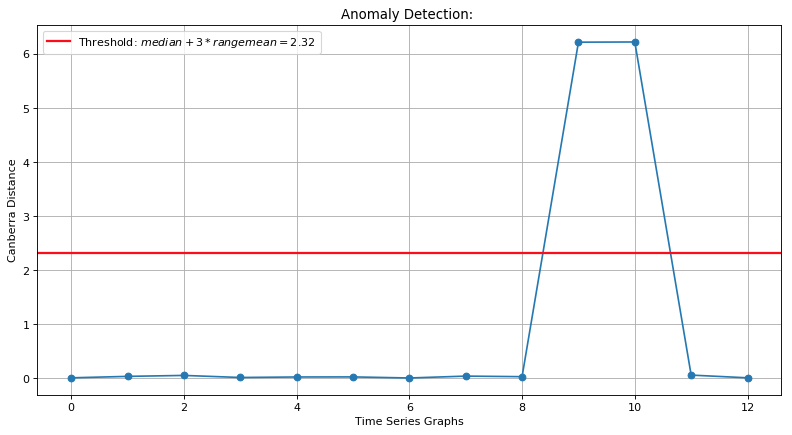
\includegraphics[height=0.6\linewidth,width=\linewidth]{fig/netsimile/anomalie_2}
	\caption{Ausrei�er Score der vollst�ndigen Graphen mit gewichteten Kanten}
	\label{img:netsimile:anomalie_2}
\end{figure}

\workTodo{Bin mir nicht sicher zu welchen Elementen die Canbarra Distanz berechnet wird.}. Des Weiteren wurde ein neuer Parameter eingef�hrt. �ber diesen kann gesteuert werden zu wie vielen vorg�nger Abschnitten die Distanz berechnet werden soll. Dadurch kann gesteuert werden wie schnell ein Algorithmus vergisst. Eine Auflistung der Parameter des Algorithmus ist in \autoref{table:parmeterNeti} zu sehen.


Um zu untersuchen, wie gut der Algorithmus funktioniert, wurde er auf Zeitreihen getestet. Als Testdaten   wurden, ein und zweidimensionale Zeitreihen der Numenta Gruppe verwendet. Diese Zeitreihen enthalten verschiedene Ausrei�er Typen, auf deren Erkennung der Algorithmus getestet wurde. Die Qualit�t der Ausrei�ererkennung wurde  mithilfe eines Punktesystem bewertet. Dabei bedeuteten 0 Punkte, Ausrei�er nicht erkannt und 4 Punkte bedeuteten Ausrei�er sehr gut erkannt. Die Parameter, welche f�r die Tests gew�hlt werden mussten, werden in \autoref{table:parmeterNeti} beschrieben.\\

\begin{table}[H]
	\centering
	\begin{tabular}{p{0.42\linewidth}|p{0.37\linewidth}|P{0.05\linewidth}|P{0.05\linewidth}}
		\toprule
		\textbf{Ausrei�er Typ}& \textbf{Datei Name}&
		\textbf{1D}&\textbf{2D}\\
		\midrule
		Einzelne Peaks & anomaly-art-daily-peaks & **& -\\
		\midrule
		Zunahme an Rauschen & anomaly-art-daily-increase-noise &****& ***\\
		\midrule
		Signal Drift & anomaly-art-daily-drift &**& -\\
		\midrule
		Kontinuierliche Zunahme der Amplitude& art-daily-amp-rise & ****& ***\\
		\midrule
		Zyklus mit h�herer Amplitude & art-daily-jumpsup &****& *\\
		\midrule
		Zyklus mit geringerer Amplitude & art-daily-jumpsdown & ****& -\\
		\midrule
		Zyklus-Aussetzer & art-daily-flatmiddle &****& ***\\
		\midrule
		Signal-Aussetzer & art-daily-nojump & ****& ***\\
		\midrule
		Frequenz�nderung & anomaly-art-daily-sequence-change &****& ***\\
		\bottomrule
	\end{tabular}
	\caption{Netsimile Time Series Perfomance}
	\label{table:performanceNeti}
\end{table}

\autoref{table:performanceNeti} zeigt die Ergebnisse der Tests. Es ist zu erkennen, dass die Qualit�t der Ausrei�er-Erkennung im eindimensionalen Fall sehr gut ist. Bei der Zeitreihe "Einzelne Peaks" werden lediglich stark abweichende Peaks erkannt. Weniger stark abweichende Peaks werden nicht erkannt. Des Weiteren wird beim Signal Drift lediglich der Anfang des Ausrei�ers detektiert. Aus diesem Grund wurde eine Bewertung mit zwei Sternen vergeben. Bei der Betrachtung der Graphiken in \autoref{sec:appendix_net_two} ist zu erkennen, dass das sechste oder siebte Intervall der Zeitreihe h�ufig als Ausrei�er markiert wird. Der Grund hierf�r ist, das bei einer Fenstergr��e von f�nf f�r die ersten f�nf Abschnitte kein Ausrei�er Score berechnet wird. Dadurch ist die Standardabweichung zu Beginn sehr niedrig wodurch Abschnitte schnell als Ausrei�er gekennzeichnet werden. Dieser Umstand wurde bei der Bewertung in \autoref{table:performanceNeti} nicht ber�cksichtigt. Im zweidimensionalen Fall ist die Qualit�t der Ausrei�er-Erkennung etwas durchwachsener. Auffallend ist, dass Zyklen mit h�herer und niedriger Amplitude nicht als Ausrei�er erkannt werden. Insbesondere ist dies auff�llig, da diese Ausrei�er Typen �blicherweise zuverl�ssig erkannt werden (vgl. \autoref{sec:rw-gl}).  Au�erdem ist der Algorithmus im zweidimensionalen Fall nicht mehr dazu in der Lage Signal Drifts zu erkennen. Andere Ausrei�er Typen k�nnen durch den Algorithmus weiterhin erkannt werden, jedoch oftmals nicht mit der selben Qualit�t. Die vollst�ndigen Ergebnisse zu den Test k�nnen in \autoref{sec:appendix_net_original} und \autoref{sec:appendix_net_two} eingesehen werden. 

\begin{table}[H]
	\centering
	\begin{tabular}{p{0.13\linewidth}|p{0.815\linewidth}}
		\toprule
		\textbf{Parameter}& \textbf{Beschreibung}\\
		\midrule
		Periodizit�t & Wie in \autoref{sec:trsnsNeti} \workTodo{Referenz sollte glaube ich autoref -> sec:trsnsNeti sein} erl�utert muss die Zeitreihe in kleinere Intervalle aufgegliedert werden. �ber diesen Parameter wird die Gr��e der Intervalle gesteuert. F�r die Tests wurde der Parameter auf 288 gesetzt, da es sich hierbei um die Saisonalit�t der Zeitreihen handelt.\\
		\midrule
		Fenstergr��e & Wie in \autoref{sec:optiNeti} erkl�rt, bestimmt dieser Parameter die Anzahl der vorangegangenen Abschnitte zu welchen die Canberra Distanz berechnet wird. Dieser Parameter wurde f�r die Tests auf 5 gesetzt.\\
		\midrule
		Abweichung & Legt fest ab wann es sich bei einem Abschnitt um einen Ausrei�er handelt. Der Parameter wurde f�r die Tests auf 3 gesetzt. Bedeutet wenn der Ausrei�er Score um das dreifache der Standardabweichung vom Durchschnitt abweicht, wird der Abschnitt als Ausrei�er gekennzeichnet.\\
		\bottomrule
	\end{tabular}
	\caption{Parameter Netsimile Zeitreihen}
	\label{table:parmeterNeti}
\end{table}


\workTodo{Die beiden Tabellen zusammenf�hren}
%\begin{table}[H]
%	\centering
%	\begin{tabular}{p{0.18\linewidth}|p{0.19\linewidth}|P{0.05\linewidth}|p{0.35\linewidth}|p{0.09\linewidth}}
%		\bottomrule
%		\textbf{Ausrei�er Typ}& \textbf{Datei Name}&
%		\textbf{1D}&\textbf{Beschreibung}&\textbf{Laufzeit}\\
%		\midrule
%		Einzelne Peaks & anomaly-art-daily-peaks & **& Zwei gemeinsame Peaks werden erkannt, Einzelne eher schlecht
%		&61min\\
%		\midrule
%		Zunahme an Rauschen & anomaly-art-daily-increase-noise &****& Ausrei�er wird erkannt&51\\
%		\midrule
%		Signal Drift & anomaly-art-daily-drift &**& Nur zwei von vier Ausrei�er werden erkannt
%		Die letzten zwei werden also normal definiert
%		&57min\\
%		\midrule
%		Kontinuierliche Zunahme der Amplitude& art-daily-amp-rise & ****& Ausrei�er werden erkannt
%		&54min\\
%		\midrule
%		Zyklus mit h�herer Amplitude & art-daily-jumpsup &****& Ausrei�er werden erkannt
%		&50\\
%		\midrule
%		Zyklus mit geringerer Amplitude & art-daily-jumpsdown & ****& Ausrei�er werden erkannt
%		&51min\\
%		\midrule
%		Zyklus-Aussetzer & art-daily-flatmiddle &****& Ausrei�er werden erkannt
%		&62min\\
%		\midrule
%		Signal-Aussetzer & art-daily-nojump & ****& Ausrei�er werden erkannt
%		&65min\\
%		\midrule
%		Frequenz�nderung & anomaly-art-daily-sequence-change &****& Ausrei�er werden erkannt
%		&49min\\
%		\bottomrule
%	\end{tabular}
%	\caption{Urspr�nglicher Netsimile Performance}
%	\label{table:performanceNeti}
%\end{table}

\workTodo{Die Bilder noch einordnen bspw. im Anhang. Im Text darauf verweisen. }

Dadurch ist die Ausrei�ererkennung von Zeitreihen in Graphen nicht m�glich. F�gt man die Gewichtung als weiteres Feature hinzu, wird hier eine erste Betrachtung der Ausrei�er m�glich. Der Graph 10 wird hier wie erhofft als Ausrei�er identifiziert.


\workTodo{bis hierhin gilt der letzte Kommentar}


\newpage
\section{MIDAS}
\label{sec:midas}
\workTodo{In diesem Kapitel werden grundlegende Themen behandelt, die im Rahmen des Forschungsprojekts zum Verst�ndnis der Ausrei�er-Erkennung in Graphen gedient haben.}


Erst erkl�ren wie der MIDAS funktioniert. Und zum Laufen gebracht mit Graphen �ber die Zeit ENRON \& DARPA. Im Anschluss auf Zeitreihendaten angewendet.


\subsection{Grundlagen}
\label{sec:mc-gl}
\workTodo{Einf�hrung in den Algorithmus, NodeHash- sowie EdgeHash-Funktionen beschreiben}

MIDAS, Eng. \textit{Microcluster-Based Detector of Anomalies in Edge Streams}, steht f�r einen Algorithmus, der pl�tzlich auftretende Ausbr�che von Aktivit�ten in einem Netzwerk bzw. Graphen erkennt. Dieses vermehrte Auftreten von Aktivit�ten zeigt sich durch viele sich wiederholende Knoten- und Kantenpaare in einem sich zeitlich entwickelnden Graphen, die Mikrocluster bezeichnet werden. Mikrocluster bestehen demnach aus einem vermehrten Vorkommen eines einzigen Quell- und Zielpaares bzw. einer Kante $(u,v)$  \workTodo{Folgender Absatz kann vor der Beschreibung des Algorithmus eingef�gt werden, wie im Paper auch} Dies geschieht in Echtzeit, wobei jede Kante in konstanter Zeit und Speicher verarbeitet wird. In der Theorie garantiert er eine False-positive-Wahrscheinlichkeit und ist durch einen 162 bis 644 mal schnelleren Ansatz, sowie einer 42\% bis 48\% h�here Genauigkeit, im Hinblick auf die AUC, sehr effektiv. \citep[vgl.][S.~1]{MIDAS}

Anwendungsf�lle f�r MIDAS sind die Erkennung von Anomalien in Computer-Netzwerken, wie SPAM oder DoS-Angriffe oder Anomalien in Kreditkartentransaktionen.


\subsubsection{Count-Min-Sketch}
\label{sec:mc-gl-cms}
Damit die relevanten Informationen f�r den Algorithmus mit einem konstanten Speicher verarbeitet werden, wird Count-Min-Sketch genutzt, dass eine Streaming-Datenstruktur mithilfe der Nutzung von Hash-Funktionen entspricht. Count-Min-Sketch z�hlt somit die Frequenz einer Aktivit�t bei Streaming-Daten. Diese Datenstruktur hat ebenfalls den Vorteil, dass man zu Beginn keine Kenntnis �ber die Anzahl an Quell- und Zielpaaren haben muss. \citep{CMS04}

MIDAS verwendet zwei Arten von CMS. Die erste Variante $s_{uv}$ wird als die Anzahl an Kanten von $u$ zu $v$ bis zum aktuellen Zeitpunkt $t$ definiert. Durch die CMS-Datenstruktur werden alle Z�hlungen von $s_{uv}$ approximiert, sodass jederzeit eine ann�hernde Abfrage $\hat{s}_{uv}$ erhalten werden kann.
Die zweite Variante $a_{uv}$ wird als die Anzahl an Kanten  von $u$ zu $v$ im aktuellen Zeitpunkt $t$ definiert. Dieser CMS ist identisch zu $s_{uv}$, wobei bei jedem �bergang zum n�chsten Zeitpunkt die Datenstruktur zur�ckgesetzt wird. Dadurch resultiert aus dem CMS f�r den aktuellen Zeitpunkt die ann�hernde Abfrage $\hat{a}_{uv}$. \citep[vgl.][S.~3]{MIDAS}


\subsubsection{Erkennung von Mikrocluster}
\label{sec:mc-gl-dm}

Mithilfe der N�herungswerte $\hat{s}_{uv}$ und $\hat{a}_{uv}$ ist das Detektieren von Mikroclustern m�glich. Hierzu wird der mittlere Pegel \workTodo{andere �bersetzung f�r mean level?} (\dah die durchschnittliche Rate mit der Kanten erscheinen) betrachtet. Es wird hierbei angenommen, dass dieser f�r den aktuellen Zeitpunkt (\zB $t = 10$) �quivalent ist zu dem vor dem aktuellen Zeitpunkt ($t < 10$). Dadurch wird die Annahmen vermieden, dass die Daten auf einer bestimmten zugrundeliegenden Verteilung basieren oder Stationarit�t �ber die Zeit aufweisen.
\\
\\
Durch die genannte Annahme lassen sich vergangene Kanten in zwei Klassen einteilen. Eine f�r den aktuellen Zeitpunkt $t = 10$ und eine f�r alle vergangenen Zeitpunkte $t < 10$. Hierbei betr�gt die Anzahl der Ereignisse zum Zeitpunkt $t = 10$ $a_{uv}$ und die Anzahl der Kanten in vergangenen Zeitpunkten $t < 10$ ist $s_{uv} - a_{uv}$.
\\
\\
Die Auswertung der Daten kann mithilfe des chi-squared goodnes-of-fit test erfolgen. Hierbei wird die Summe der Klassen $t = 10$ und $t < 10$ f�r $\frac{(\text{beobachtet} - \text{erwartet})^2}{\text{erwartet}}$ bestimmt. Bei einer Gesamtanzahl von $s_{uv}$ Kanten ergibt sich, auf Basis eines mittleren Pegels \workTodo{wie oben andere bezeichnung?}, f�r $t = 10$ eine erwartete Anzahl von $\frac{s_{uv}}{t}$ Kanten \workTodo{oder ereignisse?}. Analog hierzu ergibt sich f�r $t < 10$ eine erwartete Anzahl an $\frac{t - 1}{t}s_{uv}$ vergangenen Kanten. Daraus ergibt sich f�r die chi-squared Statistik \cite[vgl.][S.~3]{MIDAS}:

\begin{align}
	\chi^2 &= \frac{\left(\text{beobachtet}_{(t = 10)} - \text{erwartet}_{(t = 10)}\right)^2}{\text{erwartet}_{(t = 10)}} \nonumber \\
	&+ \frac{\left(\text{beobachtet}_{(t < 10)} - \text{erwartet}_{(t < 10)}\right)^2}{\text{erwartet}_{(t < 10)}} \nonumber \\
	&= \frac{\left(a_{uv} - \frac{s_{uv}}{t}\right)^2}{\frac{s_{uv}}{t}} + \frac{\left(\left(s_{uv} - a_{uv}\right) - \frac{t - 1}{t}s_{uv}\right)^2}{\frac{t - 1}{t}s_{uv}} \nonumber \\
	&= \frac{\left(a_{uv} - \frac{s_{uv}}{t}\right)^2}{\frac{s_{uv}}{t}} + \frac{\left(a_{uv} - \frac{s_{uv}}{t}\right)^2}{\frac{t - 1}{t}s_{uv}} \nonumber \\
	&= \left(a_{uv} - \frac{s_{uv}}{t}\right)^2\frac{t^2}{s_{uv}(t - 1)}
	\label{eqn:midas:chi2}
\end{align}

Die Gr��en $a_{uv}$ und $s_{uv}$ k�nnen, mithilfe der CMS-Datenstruktur, approximiert werden. Daraus ergibt sich, unter Verwendung der approximierten Gr��en $\hat{a}_{uv}$ und $\hat{s}_{uv}$, der folgende Anomaly Score \cite[vgl.][S.~4]{MIDAS}:

\begin{equation}
	score((u,v,t)) = \left(\hat{a}_{uv} - \frac{\hat{s}_{uv}}{t}\right)^2\frac{t^2}{\hat{s}_{uv}(t - 1)}
	\label{eqn:midas:score}
\end{equation}

Mithilfe des in \autoref{eqn:midas:score} angegeben Anomaly Score l�sst sich eine neue Kante $(u,v)$ zum Zeitpunkt $t$ bewerten. Dieser wird in einem bin�ren Entscheidungsverfahren verwendet, um zu bestimmen, ob es sich bei einer neuen Kante um Anomalie handelt oder nicht. Die Wahrscheinlichkeit von false positive Ergebnissen soll hierbei nicht einen benutzerdefinierten Schwellenwert $\epsilon$ �bersteigen. CMS-Datenstrukturen mit einer angemessenen Gr��e besitzen die Eigenschaft, dass die Approximationen $\hat{a}_{uv}$, f�r beliebige $\epsilon$ und $\nu$, folgende Vorschrift mit einer Wahrscheinlichkeit von mindestens $1 - \frac{\epsilon}{2}$ erf�llen:

\begin{equation}
	\hat{a}_{uv} \leq a_{uv} + \nu \cdotp N_t
\end{equation}

$N_t$ beschreibt hierbei die Anzahl an Kanten zum Zeitpunkt $t$. Eine weitere Eigenschaft der CMS-Datenstrukturen ist, dass diese die tats�chlichen Anzahl an Kanten nur �berbewerten k�nnen:

\begin{equation}
	s_{uv} \leq \hat{s}_{uv}
\end{equation}

Der in \autoref{eqn:midas:score} gegebene Score kann wie folgt angepasst werden:

\begin{equation}
	\~{a}_{uv} = \hat{a}_{uv} - \nu N_t
\end{equation}

Daraus l�sst sich die in \autoref{eqn:midas:chi2} gegebene Statistik anpassen:

\begin{equation}
	\tilde{\chi}^2 = \left(\tilde{a}_{uv} - \frac{s_{uv}}{t}\right)^2\frac{t^2}{s_{uv}(t - 1)}
	\label{eqn:midas:chi2angepasst}
\end{equation}

Bei Verwendung der Teststatistik in \autoref{eqn:midas:chi2angepasst} und eines Schwellenwertes von $\chi^2_{1 - \frac{\epsilon}{2}}(1)$ ergibt sich eine Wahrscheinlichkeit f�r ein false positive Ergebnis von h�chstens $\epsilon$:

\begin{equation}
	P\left(\tilde{\chi}^2 > \chi^2_{1 - \frac{\epsilon}{2}}(1)\right) < \epsilon
	\label{eqn:midas:prob}
\end{equation}

Der Term $\chi^2_{1 - \frac{\epsilon}{2}}(1)$ beschreibt hierbei das $1 - \frac{\epsilon}{2}$-Quantil.

\subsubsection{MIDAS-R}
Bei dem MIDAS-R Algorithmus handelt es sich um eine Erweiterung des MIDAS Algorithmus. Das R steht hierbei f�r den Relationalen Ansatz des MIDAS-R Algorithmus. Dabei wird versucht die r�umliche oder zeitliche Verkn�pfung zwischen Kanten st�rker zu ber�cksichtigten. Es werden hierzu zwei neue Konzepte eingef�hrt \citep[vgl.][S.~4]{MIDAS}.

\textbf{Temporal Relations: }Durch diesen Ansatz soll der Algorithmus mehr zeitliche Flexibilit�t erhalten. Dabei sollen Kanten aus der j�ngsten Vergangenheit auch in einem neuen Zeitabschnitt ber�cksichtigt werden. Allerdings reduziert um eine bestimmte Gewichtung. Anstatt die CMS Datenstruktur nach jedem Zeitabschnitt zu reseten, werden die Gewichte hierbei um einen bestimmten Prozentsatz reduziert \citep[vgl.][S.~4]{MIDAS}.

\textbf{Spatial Relations: }Hierbei werden zwei neue Features eingef�hrt um verschiedene Ausrei�er-Typen identifizieren zu k�nnen. Die neuen Features werden hierbei in einer CMS Datenstrukturen gespeichert. Der Algorithmus speichert demzufolge diese drei Features:

\begin{description}
	\item[$ $]\hfill\\ Anzahl an Kanten zwischen Knoten u un Knoten v. Dieses Feature wird auch vom MIDAS Algorithmus verwendet.
	\item[$ $]\hfill\\ Gesamtanzahl an Nachbarknoten eines Knoten u.
	\item[$  $]\hfill\\ Aktuelle Anzahl an Nachbarknoten eines Knoten u.
\end{description}

Aus diesen drei Features wird anschlie�end ein Ausrei�er Score abgeleitet.
 \citep[vgl.][S.~5]{MIDAS}


\section{Ausrei�er-Erkennung in Graphen}
\label{sec:m-ex}
\workTodo{ausformulieren}

\begin{figure}[H]
	\centering
	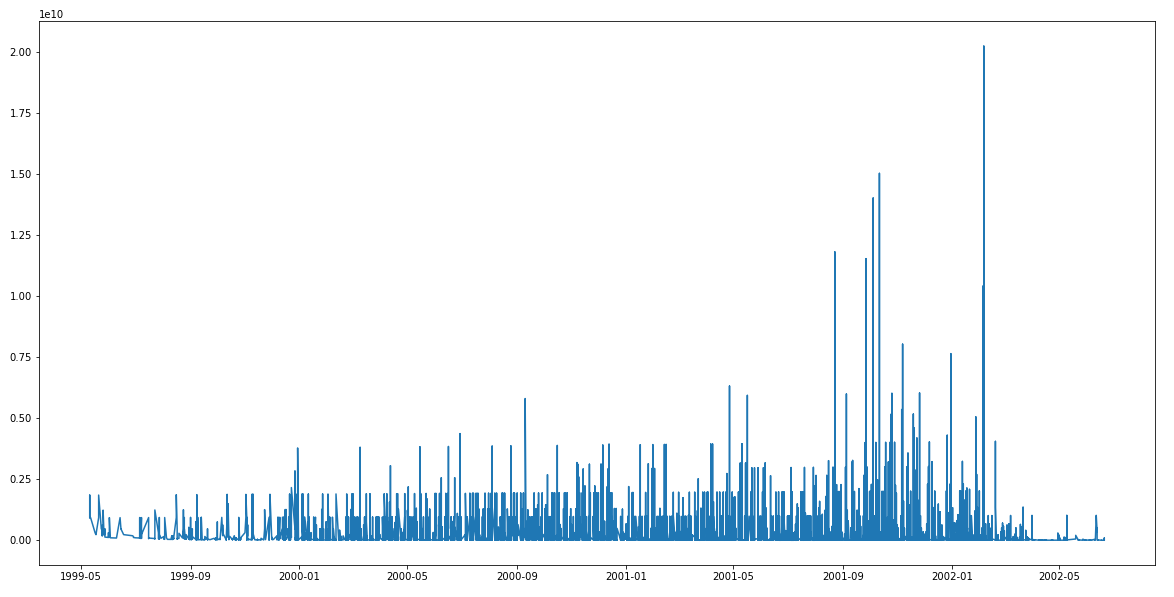
\includegraphics[height=0.6\linewidth,width=\linewidth]{fig/midas/Enron_Anomaly}
	\caption{Der Ausrei�er-Score �ber die Zeit beim ENRON-Datensatz}
	\label{img:midas:enron_anomaly}
\end{figure}



\begin{figure}[H]
	\centering
	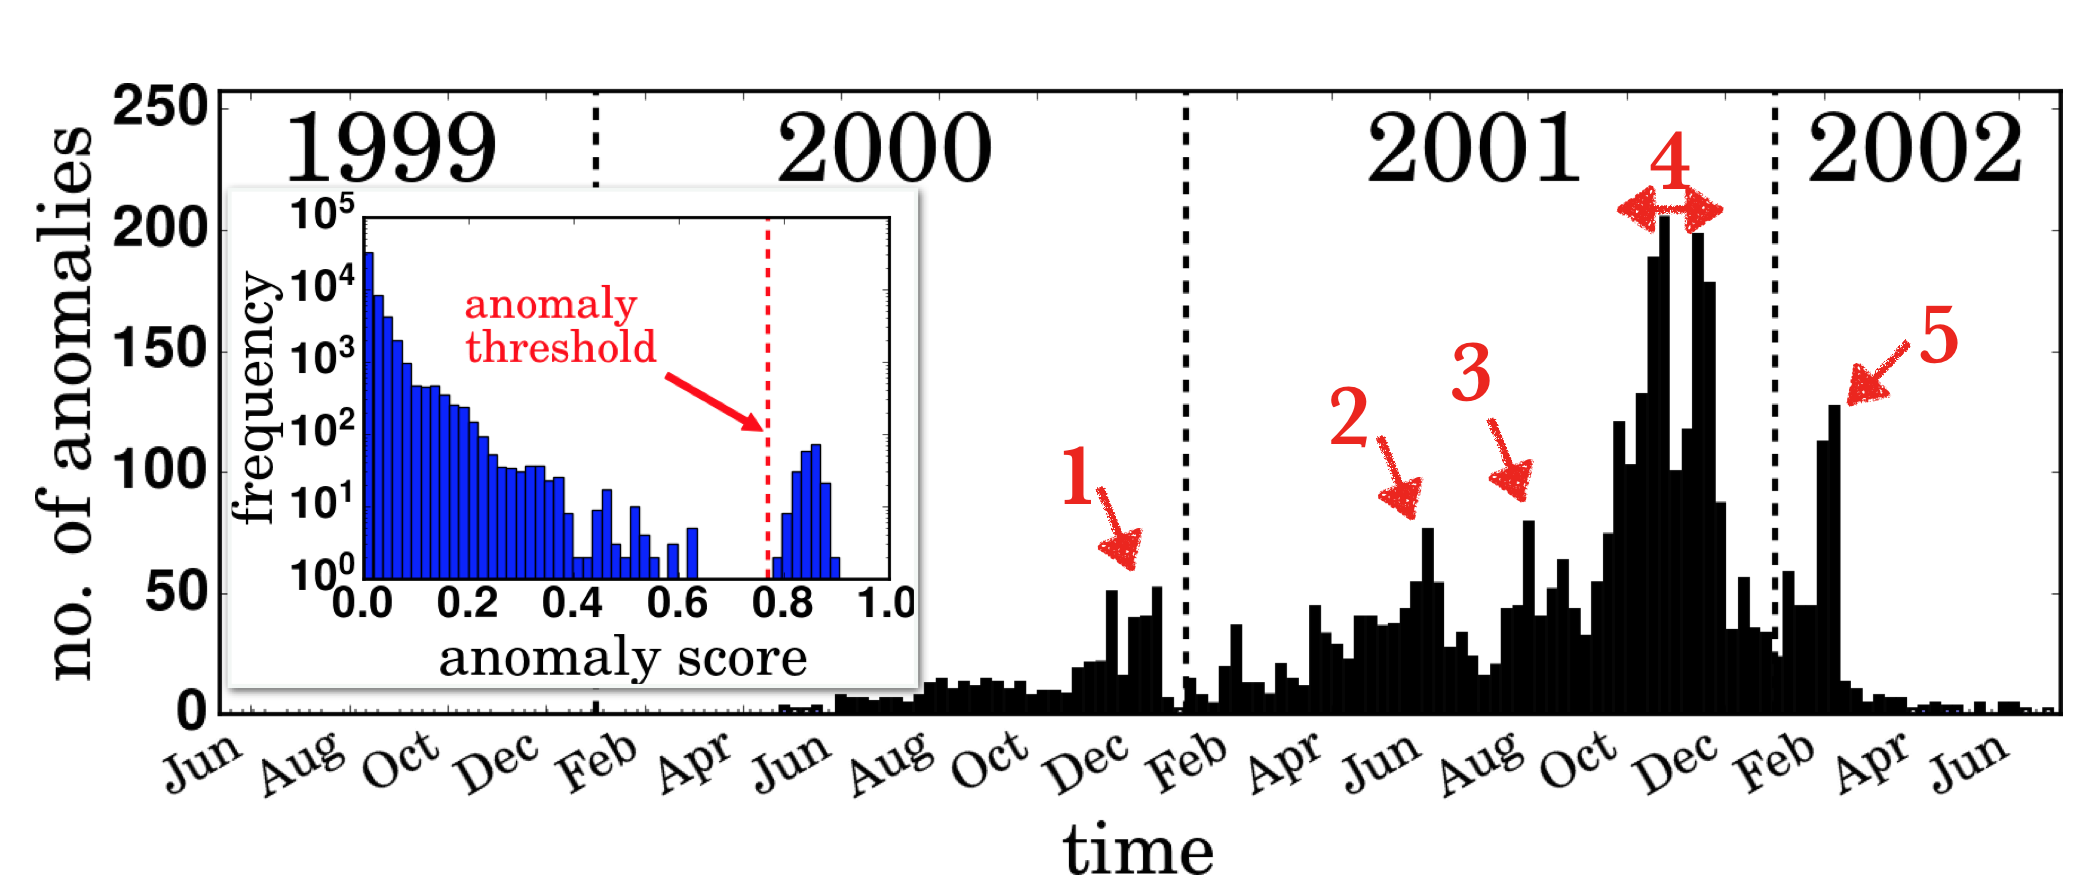
\includegraphics[height=0.4\linewidth,width=\linewidth]{fig/midas/Enron_Label}
	\caption{Die Ausrei�er des SEDANSPOT-Algorithmus}
	\label{img:midas:enron_label}
\end{figure}

Die Herausforderung geeignete \textit{labels} f�r die Datens�tze zu finden wird in zwei Schritten einged�mmt. 

Zum einen werden Erkenntnisse aus dem Schaubild des SEDANSPOT-Algorithmus gewonnen \workTodo{Quelle eingeben}. Hierbei kann man sehen, dass beide Algorithmen einen �hnlichen Verlauf vorweisen. 
Im n�chsten Schritt wird die selbe Vorgehensweise wie aus dem SEDANSPOT-Paper gew�hlt und die ENRON Timeline \workTodo{Quelle einf�gen wie bei Datensatz-Kapitel} zur Erhebung von m�glichen Auswirkungen f�r die Ausrei�er hinzugezogen.

Die \autoref{tab:enrontime} bietet eine �bersicht der historischen Ereignisse, die die Ausrei�er des MIDAS-Algorithmus erkl�ren. Im Vergleich zum SEDANSPOT-Algorithmus werden mehr Ausrei�er erkannt.
  
\begin{table}[h!]
	\centering
    \begin{tabular}{p{0.05\linewidth}|p{0.89\linewidth}}
	\toprule
	1. & Aktie erreicht Allzeithoch. Federal Energy Regulatory Commission ordnet Untersuchung an.\\
	\midrule
	2. & \textbullet Viertelj�hrliche Telefonkonferenz zur Finanzsituation und erste Symptome eines Problems. \newline \textbullet \enquote{Geheimes} Treffen -- Schwarzenegger, Lay, Milken. Angebot zur Rettung der Deregulierung. \\
	\midrule
	3. & \textbullet Skilling (CEO) k�ndigt. Mitarbeiterin warnt Lay (Gr�nder) vor Pleite. Skilling verkauft seine Aktien. \newline \textbullet Enron ver�ffentlicht 618 Mio. \$ Verlust. Interessenskonflikt wird untersucht und Akten vernichtet. \\
	\midrule
	4. & \textbullet Beginn der Strafermittlung. Lay's R�cktritt \newline \textbullet Internen Ermittlung verteilt die Schuld auf F�hrungskr�fte und den Vorstand \\
	\bottomrule
\end{tabular}
	\caption{�bersicht �ber historische Ereignisse, die den Ausrei�ern zuzuordnen sind}
	\label{tab:enrontime}
\end{table}




\begin{figure}[H]
	\centering
	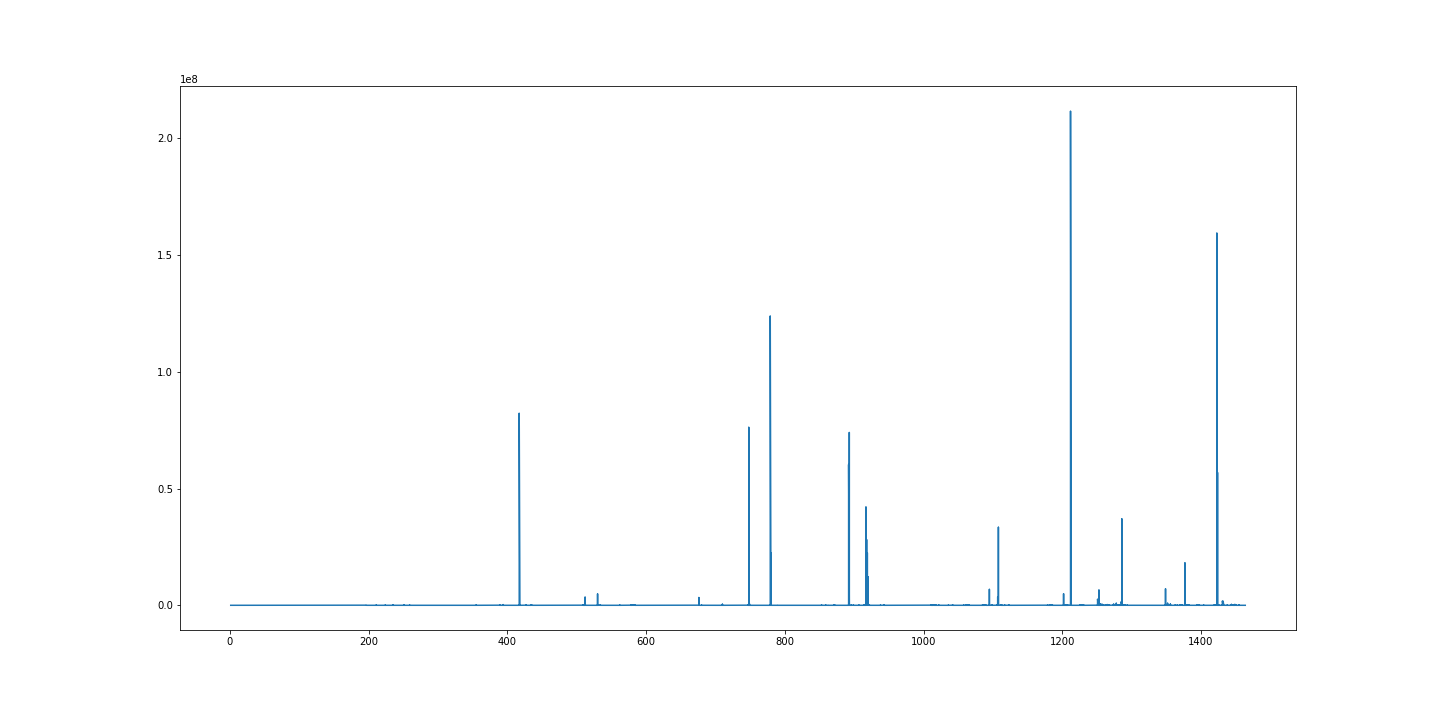
\includegraphics[height=0.6\linewidth,width=\linewidth]{fig/midas/Darpa_Anomaly}
	\caption{Der Ausrei�er-Score �ber die Zeit beim DARPA-Datensatz}
	\label{img:midas:darpa_anomaly}
\end{figure}

Bei der Anwendung des MIDAS auf dem DARPA-Datensatz sieht man sehr sch�n einzelne Ausrei�er, die entdeckt wurden. F�r diesen Datensatz gibt es, speziell f�r MIDAS entwickelt, einen \textit{ground truth}, der die \textit{labels} f�r diesen Datensatz zur Verf�gung stellt.

Bei der Berechnung der \dq Area under the Curve \dq\space f�r die ermittelten Ausrei�er-Scores wird ein Wert von $0.9172724836793507$ berechnet. Das bedeutet, dass der MIDAS-Algorithmus mit einer Wahrscheinlichkeit von ca. 91,73\% die Kanten des Datensatzes richtig klassifiziert.  

Somit kann festgehalten werden, dass MIDAS ein sehr guter Algorithmus ist bei der Erkennung von Ausrei�ern in Graphen und eine sehr hohe Genauigkeit erreicht.

\workTodo{Schwierigkeit geeignete Datens�tze zu finden, dazu gibt es ein Paper. Wenn man die Anomalyscores als gewichte nimmt, kommen Graphen in Networkx raus in denen man die anomalous nodes identifizieren kann dabei sollten es Edges sein}


\section{Ausrei�er-Erkennung in Zeitreihen}
\label{sec:resultsOTs}
\workTodo{Tabelle wie f�r Netsimile einf�gen bzgl. den verschiedenen Numenta-Datens�tzen. Bisher nicht dringlich gewesen, da MIDAS schlecht ist und wir das f�r den abstract nicht ben�tigen}

Um den MIDAS Algorithmus auf Zeitreihen anwenden zu k�nnen muss die Zeitreihe, wie in \autoref{chap:trsnsMidas} beschrieben, zun�chst in verschiedene Netzwerke umgewandelt werden. Bei den Tests konnte festgestellt werden, dass der MIDAS Algorithmus nicht dazu in der Lage ist Ausrei�er in Zeitreihen zu erkennen. Die vollst�ndigen Ergebnisse der Tests k�nnen in \autoref{chap:appendix_midas_ts} eingesehen werden. Hierbei ist jedoch der Verlauf des Ausrei�er Scores schwierig zu interpretieren. Es ist zu erkennen, das der Ausrei�er-Score zu Beginn eines jeden Abschnitts sehr hoch ist, am Ende des Abschnitts ist der Ausrei�er Score hingegen relativ niedrig. Grund hierf�r ist, das die Anzahl an Kanten zu Beginn eines Abschnittes im Verh�ltnis zu der Anzahl an Kanten aus den vorangegangenen Abschnitten deutlich niedriger ist. Im weiteren Verlauf werden weitere Kanten innerhalb des Abschnitts hinzugef�gt. Dadurch gleicht sich die Anzahl an Kanten innerhalb der Abschnitte an und der Ausrei�er Score sinkt.

Der MIDAS Algorithmus ist lediglich bei einer Zeitreihe dazu in der Lage den Ausrei�er zu identifizieren. Hierbei handelt es sich um die Zeitreihe mit erh�hter Amplitude (vgl. \autoref{img:midasTSresultJumpsup}). Durch den Ausschlag nach oben in der Zeitreihe entsteht ein Netzwerk, mit sehr hohen Gewichten. Die hohen Gewichte f�hren zu einer erh�hten Anzahl an Kanten, was schlussendlich zu einem Ausschlag des Ausrei�er Scores f�hrt. Die erh�hte Anzahl an Kanten f�hrt ebenfalls dazu das der Abschnitt mit dem Ausrei�er in der Abbildung deutlich breiter ist als die anderen. Bei anderen Ausrei�er Typen sind die Differenzen zwischen den verschiedenen Elementen der Zeitreihe nicht so gro�. Dadurch ergeben sich keinerlei hohe Kantengewichte und der Ausrei�er kann nicht erkannt werden.


\begin{figure}[h]
	\centering
	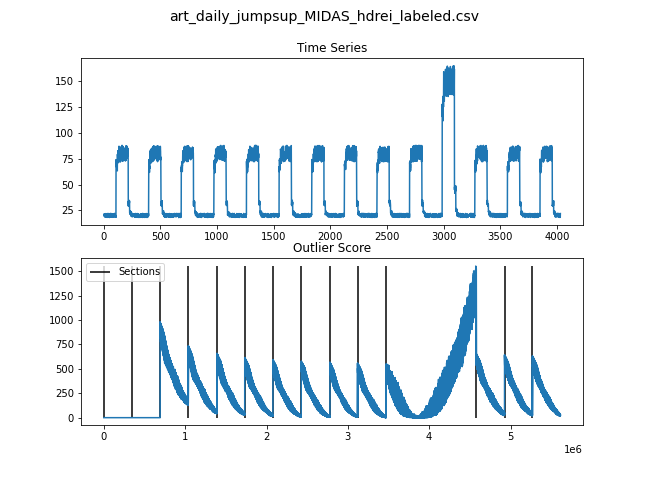
\includegraphics[width=0.5\textwidth]{fig/resultsMidasTS/art_daily_jumpsup_MIDAS_hdrei_labeled_result.png}
	\caption{MIDAS Algorithmus angewandt auf Zeitreihe mit einer erh�ten Amplitude.}
	\label{img:midasTSresultJumpsup}
\end{figure}

Teilweise f�hren die Ausrei�er auch zu besonders wenigen Kanten (vgl. \autoref{img:midasTSresultsFlatSeqChange}). Bei diesem Ausrei�er Typ sind alle Werte auf der selben Ebene. Dadurch gehen die Kantengewichte gegen Null. Dies f�hrt zu einem sehr kurzen Abschnitt in der Abbildung (Der Abschnitt wurde mit einem Pfeil markiert). \workTodo{Noch Pfeil in Graphik einf�gen} Des weiteren ergibt sich durch die Ausrei�er eine leicht ver�nderte Anzahl an Kanten in dem Abschnitt mit dem Ausrei�er (vgl. \autoref{img:midasTSresultsFlatSeqChange}). Die Abweichungen sind jedoch so gering, dass es nicht zu einem starken Anstieg des Ausrei�er Scores f�hrt.
\label{sec:resultTSwithoutMidas}

\begin{figure}[h]
	\centering
	\subfloat[Zeitreihe mit Zyklus Aussetzter]{
		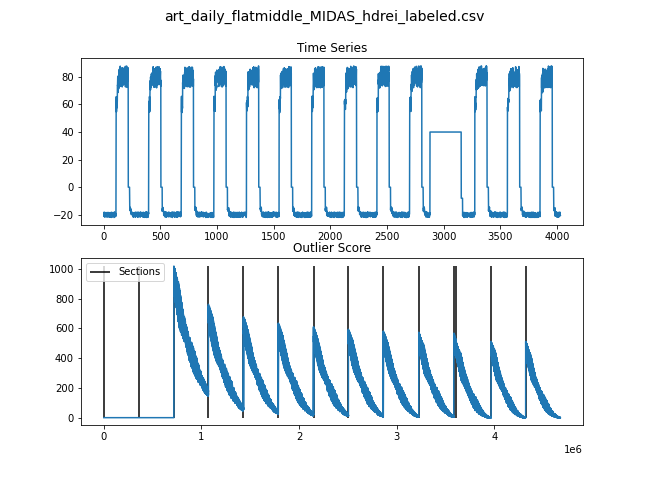
\includegraphics[width=0.5\textwidth]{fig/resultsMidasTS/art_daily_flatmiddle_MIDAS_hdrei_labeled_result.png}}
	\subfloat[Zeitreihe mit Frequenz�nderung]{
		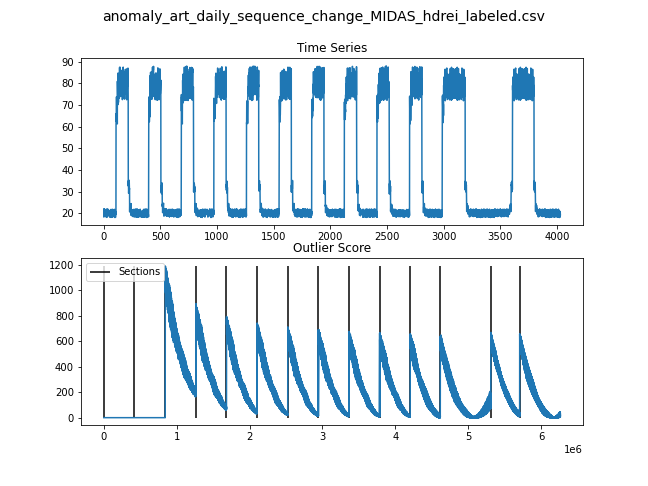
\includegraphics[width=0.5\textwidth]{fig/resultsMidasTS/anomaly_art_daily_sequence_change_MIDAS_hdrei_labeled_result.png}}
	\caption{Ausrei�er Erkennung in Zeitreihen MIDAS Algorithmus}
	\label{img:midasTSresultsFlatSeqChange}
\end{figure}

Es wurden au�erdem Tests durchgef�hrt um zu Untersuchen, wie sich der Algorithmus bei ver�nderter Fenstergr��e verh�lt (vgl. \autoref{img:midasTSresults110}). Bei den Untersuchungen in \autoref{img:midasTSresultJumpsup} und \autoref{img:midasTSresultsFlatSeqChange} wurde einer Fenstergr��e von 288 genutzt, was der Saisonalit�t der Zeitreihe entspricht. F�r dieses Experiment wurde einer Fenstergr��e von 110 verwendet. Es konnte festgestellt werden, das diese Ver�nderung keinen zus�tzlichen Nutzen erbringt. Allerdings ist der Ausschlag nach oben im Ausrei�er Score f�r die Zeitreihe mit erh�hter Amplitude noch deutlicher zu erkennen. Die anderen Ausrei�er Typen werden weiterhin nicht erkannt.

\begin{figure}[h]
	\centering
	\subfloat[Zeitreihe mit einer Frequenz�nderung]{
		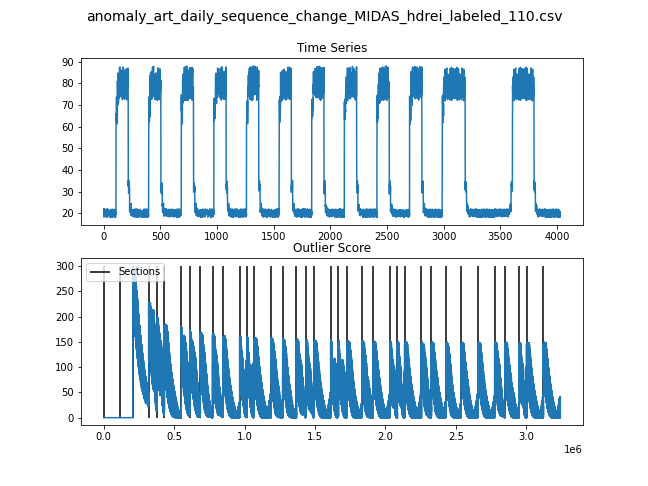
\includegraphics[width=0.5\textwidth]{fig/resultsMidasTS/anomaly_art_daily_sequence_change_MIDAS_hdrei_labeled_110_result.png}}	
	\subfloat[Zeitreihe mit erh�hter Amplitude]{
		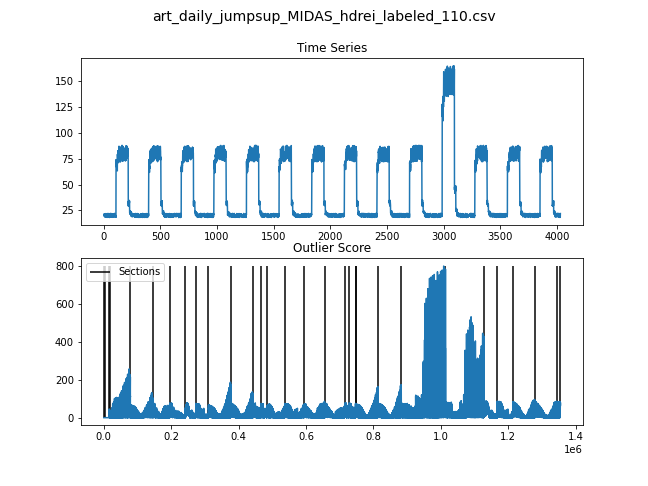
\includegraphics[width=0.5\textwidth]{fig/resultsMidasTS/art_daily_jumpsup_MIDAS_hdrei_labeled_110_result.png}}
	\caption{Ausrei�er Erkennung Zeitreihen MIDAS Algorithmus Fenstergr��e 110}
	\label{img:midasTSresults110}
\end{figure}

In einem n�chsten Schritt wurde untersucht inwiefern der MIDAS-R Algorithmus zu einer Verbesserung bei der Ausrei�er Erkennung beitragen kann (vgl. \autoref{img:midasRTSresults}). Der MIDAS-R Algorithmus ber�cksichtigt bei der Berechnung des Ausrei�er Scores f�r den aktuellen Abschnitt auch die Daten aus der j�ngsten Vergangenheit(vorangegangene Abschnitte). Aus diesem Grund erhofften wir uns durch den Einsatz des MIDAS-R Algorithmus, dass die Ausschl�ge zu beginn eines jeden Abschnitts aus bleiben, sodass Ausrei�er deutlicher hervortreten. Es konnte festgestellt werden, dass der Ausschlag des Ausrei�er Scores zu Beginn der Abschnitte deutlich kleiner ist. Jedoch steigt der Ausrei�er Score zum Ende eines jeden Abschnitts wieder an. Es konnte somit keine Signifikante Verbesserung bei der Erkennung von Ausrei�ern erreicht werden. Insbesondere da der MIDAS-R Algorithmus ebenfalls nur den Ausrei�er in der Zeitreihe mit erh�hter Amplitude anzeigt. Somit konnte festgestellt werden, dass auch die durch den MIDAS-R Algorithmus eingef�hrten Features zu keiner Verbesserung der Ergebnisse gef�hrt haben. 
\workTodo{Vielleicht k�nnte eine Verbesserung erreicht werden wenn andere Features eingef�hrt werden w�rden.}


\begin{figure}[h]
	\centering
	\subfloat[Zeitreihe mit geringerer Amplitude]{
		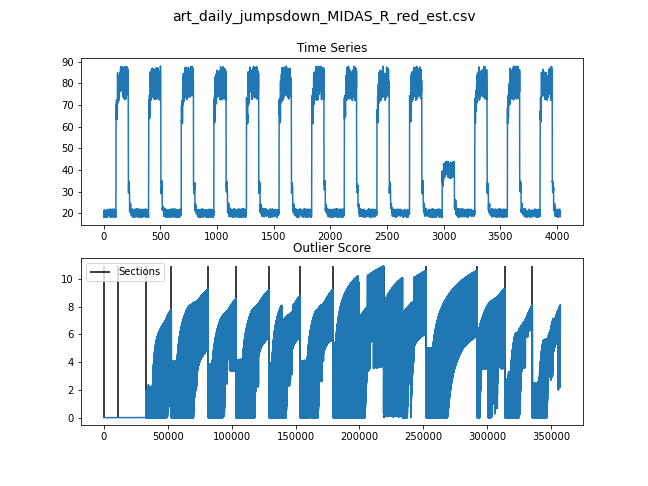
\includegraphics[width=0.5\textwidth]{fig/reultsMidasR/art_daily_jumpsdown_MIDAS_R_red_est_result}}
	\subfloat[Zeitreihe mit erh�hter Amplitude]{
		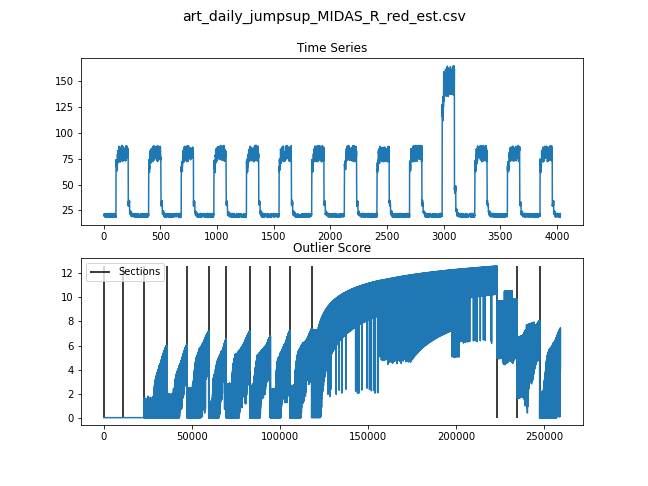
\includegraphics[width=0.5\textwidth]{fig/reultsMidasR/art_daily_jumpsup_MIDAS_R_red_est_result}}
	\caption{Ausrei�er Erkennung Zeitreihen MIDAS-R}
	\label{img:midasRTSresults}
\end{figure}



